
\section{Übertragungsleitungen}
\label{section:uebertragungsleitungen}
\begin{frame}%STARTCONTENT
Die im Sender erzeugte Sendeleistung möchte man möglichst vollständig und ohne Verluste von der Antenne abstrahlen

\end{frame}

\begin{frame}
\frametitle{Koaxialkabel}
\begin{columns}
    \begin{column}{0.48\textwidth}
    
\begin{figure}
    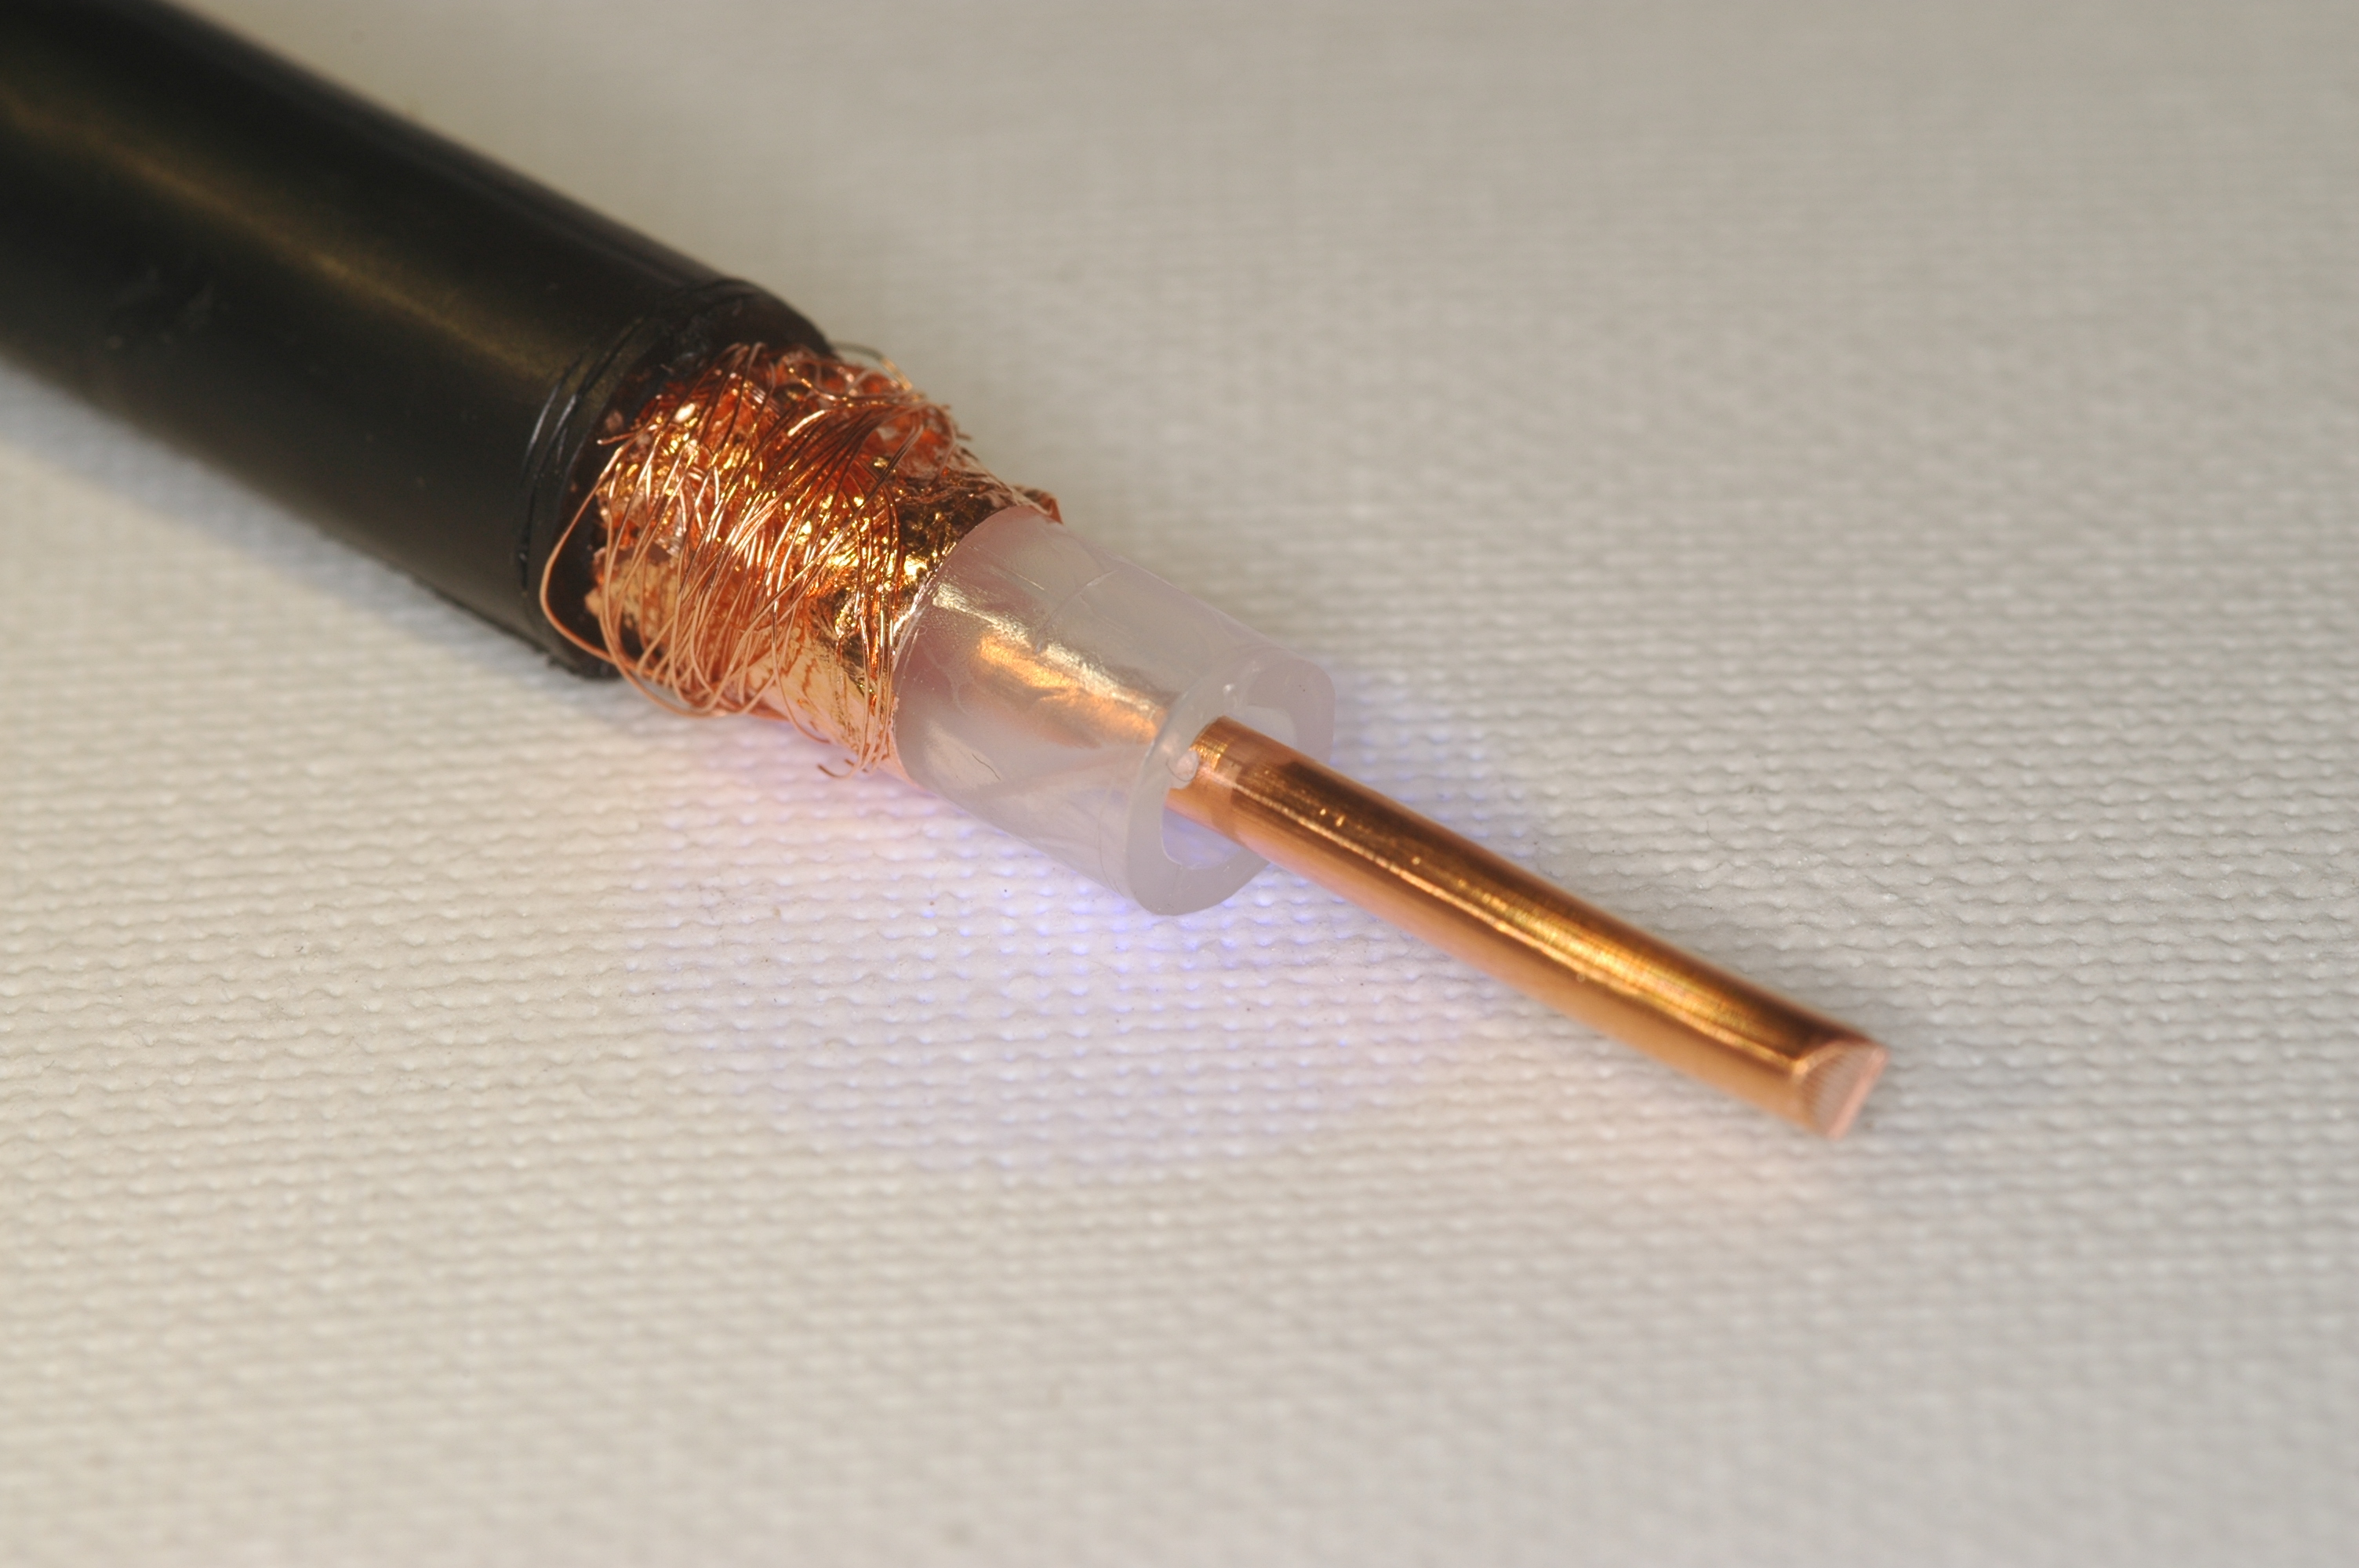
\includegraphics[width=0.85\textwidth]{foto/65}
    \caption{\scriptsize Koaxial-Kabel im Detail}
    \label{n_Koax_Detail}
\end{figure}

    \end{column}
   \begin{column}{0.48\textwidth}
       \begin{itemize}
  \item Am weitesten verbreitet
  \item Voneinander isolierter Innen- und Außenleiter
  \item Umgeben von Schutzmantel
  \item Unterschiedliche Ausführungen möglich
  \end{itemize}

   \end{column}
\end{columns}

\end{frame}

\begin{frame}
\frametitle{Unterschiedliche Koaxialkabel}

\begin{figure}
    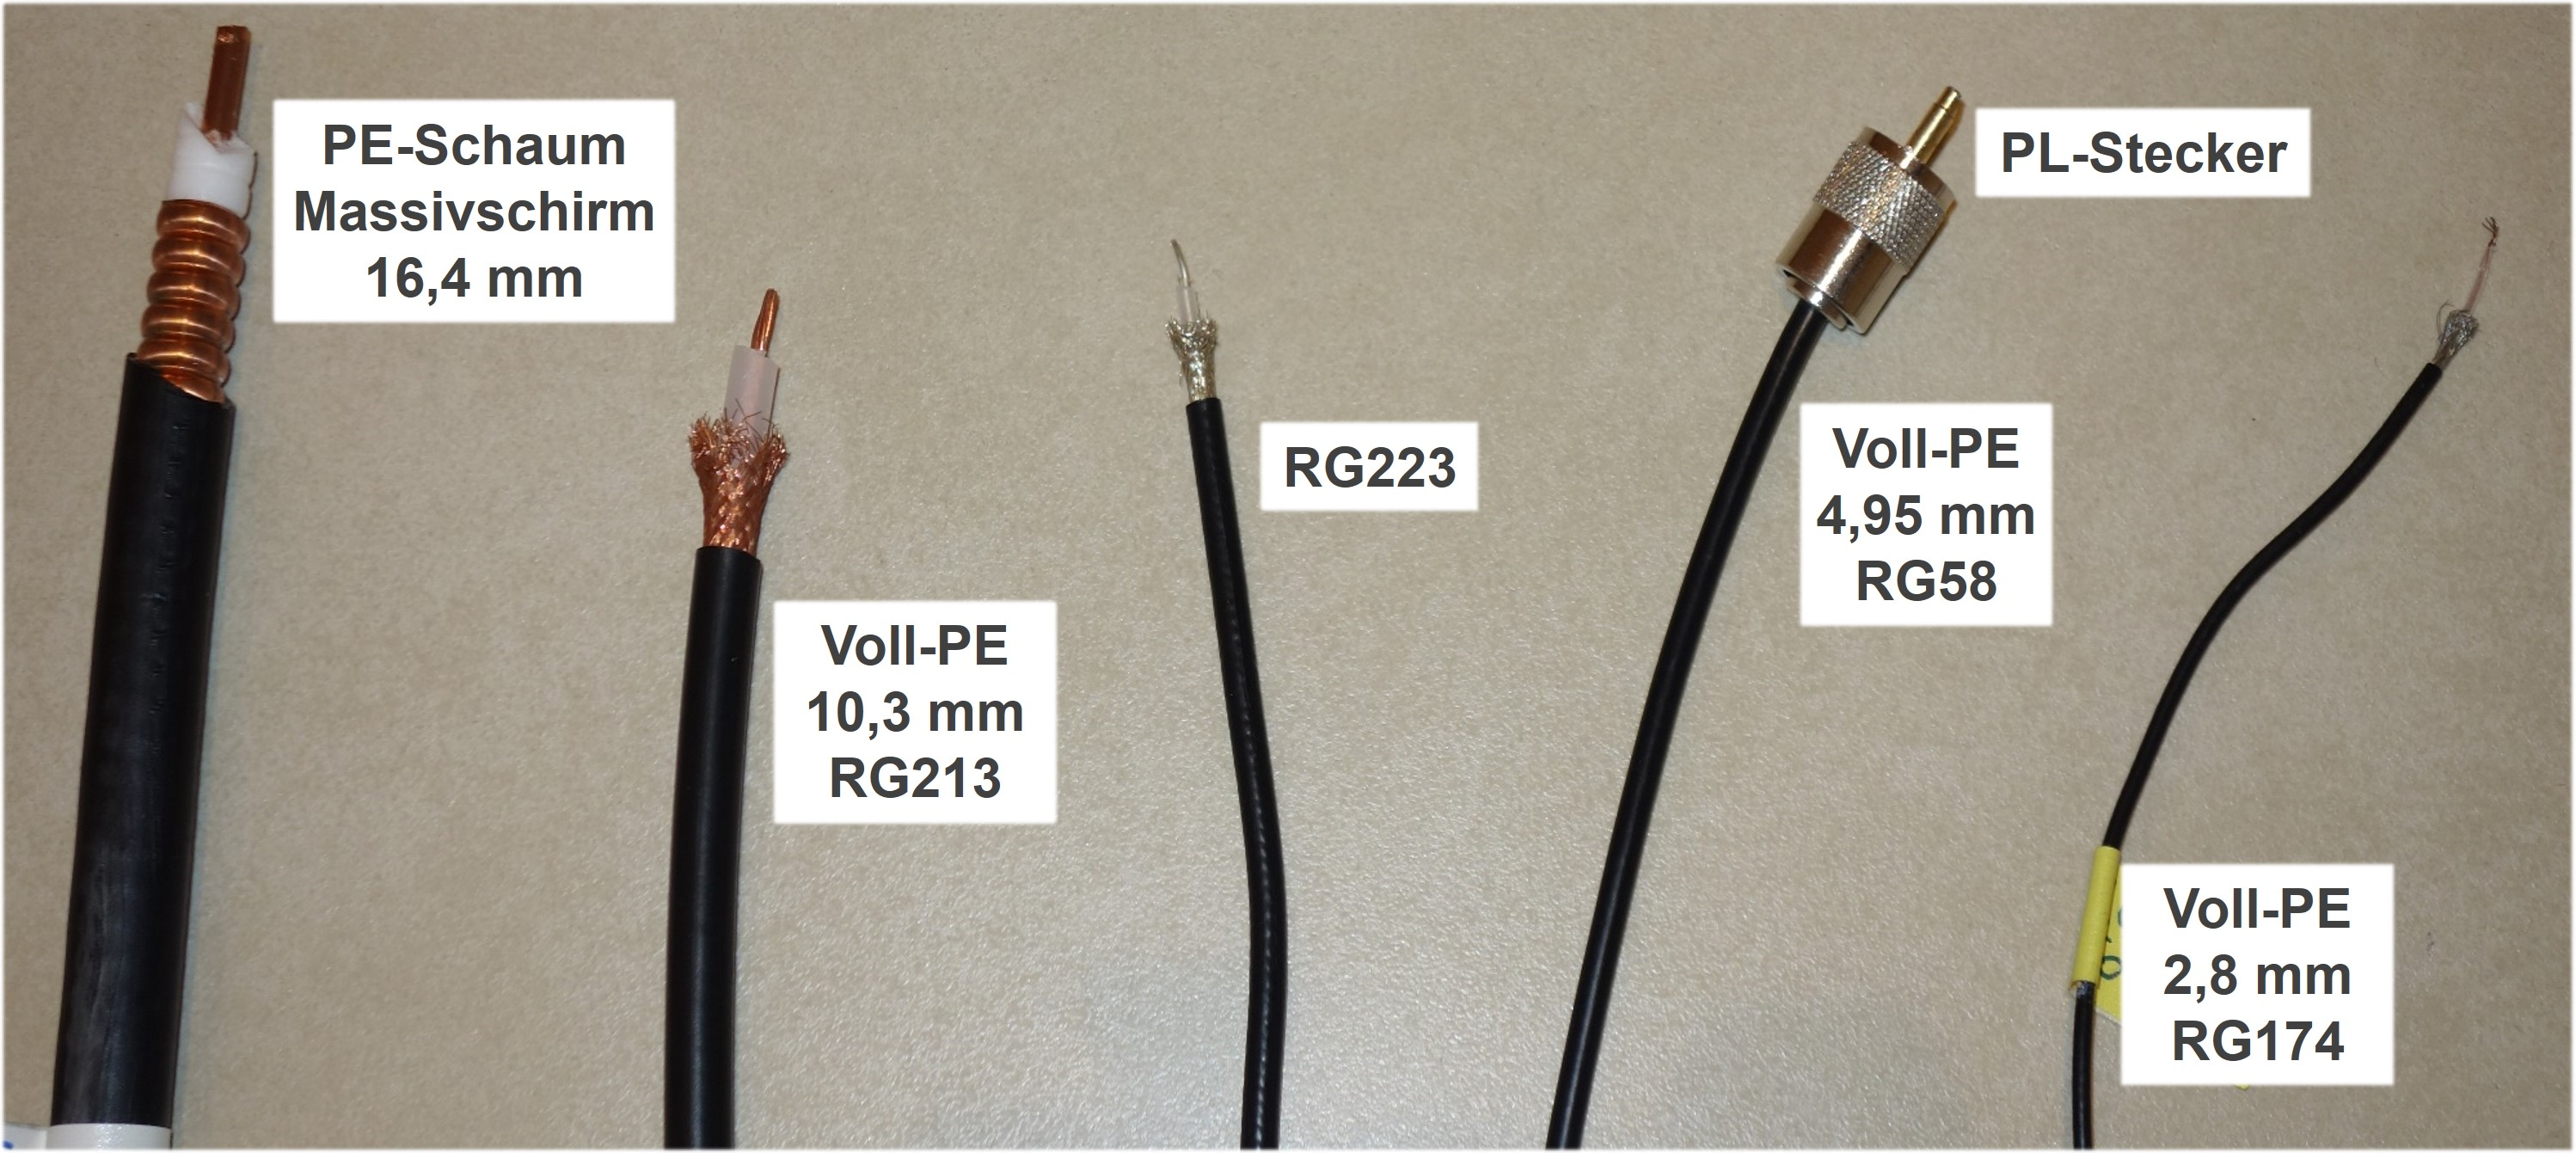
\includegraphics[width=0.85\textwidth]{foto/66}
    \caption{\scriptsize Beispiele gebräuchlicher Koaxialkabel}
    \label{n_Koaxialkabel}
\end{figure}
\end{frame}

\begin{frame}
\frametitle{Kabeldämpfung}
\begin{itemize}
  \item Im Koaxialkabel entsteht Verlust durch Umsetzung von Sendeleistung in Wärme
  \item Der Verlust wird \emph{Kabeldämpfung} genannt
  \item Messung in Dezibel (dB) je 100~m
  \item Verluste steigen mit zunehmender Länge und Frequenz
  \end{itemize}
\end{frame}

\begin{frame}
\only<1>{
\begin{QQuestion}{NG207}{Zwischen VHF/UHF-Transceiver und Antenne soll ein Koaxialkabel verwendet werden. Welche Aspekte sind neben dem richtigen Wellenwiderstand bei der Kabelauswahl zu beachten?}{Die Kabellänge hat keinen Einfluss auf die Kabeldämpfung.}
{Die Dämpfung sinkt mit zunehmender Länge und Frequenz.}
{Die Verluste steigen mit zunehmender Länge und Frequenz.}
{Die Frequenz hat keinen Einfluss auf die Kabeldämpfung.}
\end{QQuestion}

}
\only<2>{
\begin{QQuestion}{NG207}{Zwischen VHF/UHF-Transceiver und Antenne soll ein Koaxialkabel verwendet werden. Welche Aspekte sind neben dem richtigen Wellenwiderstand bei der Kabelauswahl zu beachten?}{Die Kabellänge hat keinen Einfluss auf die Kabeldämpfung.}
{Die Dämpfung sinkt mit zunehmender Länge und Frequenz.}
{\textbf{\textcolor{DARCgreen}{Die Verluste steigen mit zunehmender Länge und Frequenz.}}}
{Die Frequenz hat keinen Einfluss auf die Kabeldämpfung.}
\end{QQuestion}

}
\end{frame}

\begin{frame}
\frametitle{Wellenwiderstand}
\begin{columns}
    \begin{column}{0.48\textwidth}
    \begin{itemize}
  \item Wird in Ohm (Ω) angegeben
  \item Eigenschaft der Leitung, wie den Aufbau (z.B. Abstand zwischen Innen- und Außenleiter)
  \item Länge hat keine Auswirkung
  \end{itemize}

    \end{column}
   \begin{column}{0.48\textwidth}
       
    \pause
    \begin{itemize}
  \item Antennenanschluss von Amateurfunkgeräten: 50~Ω
  \item Koaxialkabel im Amateurfunk: 50~Ω
  \item Fernsehtechnik: 75~Ω
  \item Selten sind 60~Ω anzufinden
  \end{itemize}



   \end{column}
\end{columns}

\end{frame}

\begin{frame}
\only<1>{
\begin{QQuestion}{NG201}{Koaxialkabel weisen typischerweise Wellenwiderstände von~...}{\num{50}, \num{75} und \qty{240}{\ohm} auf.}
{\num{50}, \num{300} und \qty{600}{\ohm} auf.}
{\num{60}, \num{120} und \qty{240}{\ohm} auf.}
{\num{50}, \num{60} und \qty{75}{\ohm} auf.}
\end{QQuestion}

}
\only<2>{
\begin{QQuestion}{NG201}{Koaxialkabel weisen typischerweise Wellenwiderstände von~...}{\num{50}, \num{75} und \qty{240}{\ohm} auf.}
{\num{50}, \num{300} und \qty{600}{\ohm} auf.}
{\num{60}, \num{120} und \qty{240}{\ohm} auf.}
{\textbf{\textcolor{DARCgreen}{\num{50}, \num{60} und \qty{75}{\ohm} auf.}}}
\end{QQuestion}

}
\end{frame}%ENDCONTENT
